% \documentclass[handout]{beamer}
\documentclass{beamer}

\mode<presentation>
{
  \usetheme{ANLBlue}
  % \usefonttheme[onlymath]{serif}
  % \usetheme{Singapore}
  % \usetheme{Warsaw}
  % \usetheme{Malmoe}
  % \useinnertheme{circles}
  % \useoutertheme{infolines}
  % \useinnertheme{rounded}

  \setbeamercovered{transparent=5}
}

\usepackage[english]{babel}
\usepackage[latin1]{inputenc}
\usepackage{alltt,listings,multirow,ulem,siunitx}
\usepackage[absolute,overlay]{textpos}
\TPGrid{1}{1}
\usepackage{pdfpages}
\usepackage{ulem}
\usepackage{multimedia}
\usepackage{multicol}
\newcommand\hmmax{0}
\newcommand\bmmax{0}
\usepackage{bm}
\usepackage{comment}
\usepackage{subcaption}

% font definitions, try \usepackage{ae} instead of the following
% three lines if you don't like this look
\usepackage{mathptmx}
\usepackage[scaled=.90]{helvet}
% \usepackage{courier}
\usepackage[T1]{fontenc}
\usepackage{tikz}
\usetikzlibrary{decorations.pathreplacing}
\usetikzlibrary{shadows,arrows,shapes.misc,shapes.arrows,shapes.multipart,arrows,decorations.pathmorphing,backgrounds,positioning,fit,petri,calc,shadows,chains,matrix,mindmap}

\newcommand\vvec{\bm v}
\newcommand\bvec{\bm b}
\newcommand\bxk{\bvec_0 \times \kappa_0 \cdot \nabla}
\newcommand\delp{\nabla_\perp}

% \usepackage{pgfpages}
% \pgfpagesuselayout{4 on 1}[a4paper,landscape,border shrink=5mm]

\usepackage{JedMacros}

\newcommand{\timeR}{t_{\mathrm{R}}}
\newcommand{\timeW}{t_{\mathrm{W}}}
\newcommand{\mglevel}{\ensuremath{\ell}}
\newcommand{\mglevelcp}{\ensuremath{\mglevel_{\mathrm{cp}}}}
\newcommand{\mglevelcoarse}{\ensuremath{\mglevel_{\mathrm{coarse}}}}
\newcommand{\mglevelfine}{\ensuremath{\mglevel_{\mathrm{fine}}}}

%solution and residual
\newcommand{\vx}{\ensuremath{x}}
\newcommand{\vc}{\ensuremath{\hat{x}}}
\newcommand{\vr}{\ensuremath{r}}
\newcommand{\vb}{\ensuremath{b}}

%operators
\newcommand{\vA}{\ensuremath{A}}
\newcommand{\vP}{\ensuremath{I_H^h}}
\newcommand{\vS}{\ensuremath{S}}
\newcommand{\vR}{\ensuremath{I_h^H}}
\newcommand{\vI}{\ensuremath{\hat I_h^H}}
\newcommand{\vV}{\ensuremath{\mathbf{V}}}
\newcommand{\vF}{\ensuremath{F}}
\newcommand{\vtau}{\ensuremath{\mathbf{\tau}}}


\title{Time Integration for Atmospheric Physics}
%\subtitle{This talk: \url{http://59A2.org/files/20141212-Benchmarking.pdf}}

\author{{\bf Jed Brown} \texttt{jed@jedbrown.org} (ANL and CU Boulder)}

% - Use the \inst command only if there are several affiliations.
% - Keep it simple, no one is interested in your street address.
% \institute
% {
%   Mathematics and Computer Science Division \\ Argonne National Laboratory
% }

\date{SIAM CSE, 2015-03-16}

% This is only inserted into the PDF information catalog. Can be left
% out.
\subject{Talks}


% If you have a file called "university-logo-filename.xxx", where xxx
% is a graphic format that can be processed by latex or pdflatex,
% resp., then you can add a logo as follows:

% \pgfdeclareimage[height=0.5cm]{university-logo}{university-logo-filename}
% \logo{\pgfuseimage{university-logo}}



% Delete this, if you do not want the table of contents to pop up at
% the beginning of each subsection:
% \AtBeginSubsection[]
% {
% \begin{frame}<beamer>
%   \frametitle{Outline}
%   \tableofcontents[currentsection,currentsubsection]
% \end{frame}
% }

\AtBeginSection[]
{
  \begin{frame}<beamer>
    \frametitle{Outline}
    \tableofcontents[currentsection]
  \end{frame}
}

% If you wish to uncover everything in a step-wise fashion, uncomment
% the following command:

% \beamerdefaultoverlayspecification{<+->}

\begin{document}
\lstset{language=C}
\normalem

\begin{frame}
  \titlepage
\end{frame}

\begin{frame}{What is performance?}
  \begin{block}{}
    \begin{itemize}
    \item Accuracy
    \item Model complexity
    \item Compute Time
    \item Human Time
    \item Cost
    \end{itemize}
  \end{block}
  \begin{itemize}
  \item Terms relevant to scientist/engineer
  \item No flop/s, number of elements/time steps
  \end{itemize}
\end{frame}

\begin{frame}{Work-precision diagram: \emph{de rigueur} in ODE community}
  \begin{center}
    \includegraphics[width=0.8\textwidth]{figures/HairerWanner-WorkPrecision.png}\\
    {\scriptsize [Hairer and Wanner (1999)]}
  \end{center}
  \begin{itemize}
  \item Tests discretization, adaptivity, algebraic solvers, implementation
  \item No reference to number of time steps, number of grid points, etc.
  \end{itemize}
\end{frame}

\begin{frame}{Exascale Science \& Engineering Demands}
  \begin{itemize}
  \item Model fidelity: resolution, multi-scale, coupling
    \begin{itemize}
    \item Transient simulation is not weak scaling: $\Delta t \sim \Delta x$
    \end{itemize}
  \item Analysis using a sequence of forward simulations
    \begin{itemize}
    \item Inversion, data assimilation, optimization
    \item Quantify uncertainty, risk-aware decisions
    \end{itemize}
  \item Increasing relevance $\implies$ external requirements on time
    \begin{itemize}
    \item Policy: 5 SYPD to inform IPCC
    \item Weather, manufacturing, field studies, disaster response
    \end{itemize}
  \item ``weak scaling'' [\ldots] will increasingly give way to ``strong scaling''\\
    {\scriptsize [The International Exascale Software Project Roadmap, 2011]}
  \item ACME @ \SI{15}{\kilo\metre} scaling saturates at $<10\%$ of Titan (CPU) or Mira
    \begin{itemize}
    \item Cannot decrease $\Delta x$: SYPD would be too slow to calibrate
    \item ``results'' would be meaningless for 50-100y predictions, a ``stunt run''
    \end{itemize}
  \item \alert{\bf ACME v1 goal of 5 SYPD is pure strong scaling.}
    \begin{itemize}
    \item Many non-climate applications in same position.
    \end{itemize}
  \end{itemize}
\end{frame}

\begin{frame}{HPGMG-FE on Edison, SuperMUC, Titan}
  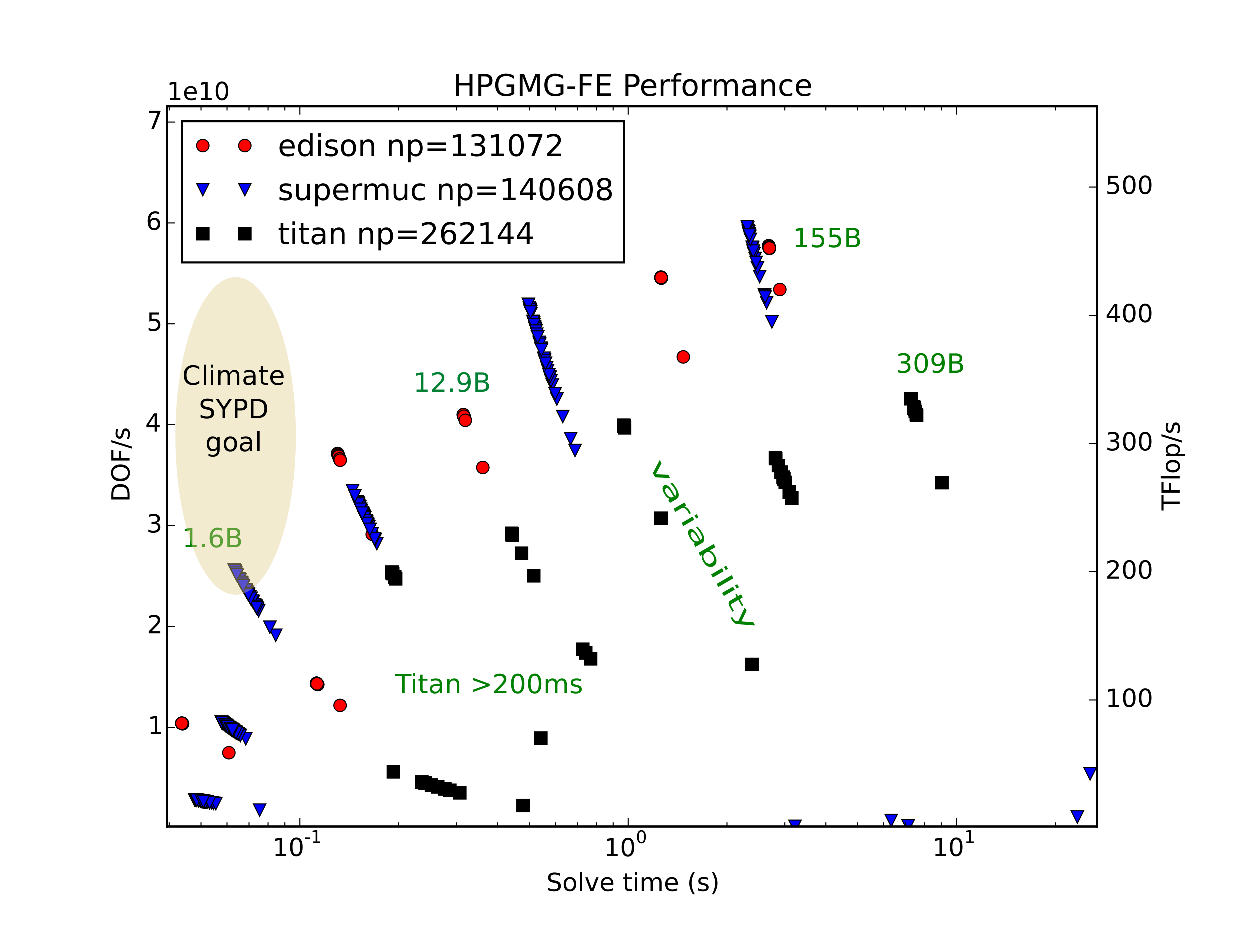
\includegraphics[width=\textwidth]{figures/hpgmg/range-edison-supermuc-titan-ann2.eps}
\end{frame}

\begin{frame}{What is Stiffness?}
  \begin{definition}[Stiffness]
    A dynamical system is \emph{stiff} if time integration efficiency is limited by stability rather than accuracy.
  \end{definition}
  \begin{itemize}
  \item Is air flow in this room stiff?
  \item<2> A property of the physical system \emph{and} quantities of interest
  \end{itemize}
\end{frame}

\begin{frame}{KiD: Kinematic Driver}
  \begin{itemize}
  \item Shipway and Hill (UK Met Office)
  \item Morrison and Gettelman (NCAR) - CAM5 microphysics
  \item Peter Caldwell (LLNL)
  \item 1D and 2D mode, diagnostic velocity
  \item Time integration methods
    \begin{itemize}
    \item Heavy use of splitting
    \item Some implicit substeps
    \end{itemize}
  \item State scattered among global variables
  \item Functions take time steps with side-effects
  \end{itemize}
\end{frame}

\begin{frame}{Accuracy of reference integrator}
  \begin{center}
    \includegraphics[width=0.8\textwidth]{figures/acme/total_surface_ppt.pdf}
  \end{center}
  \begin{itemize}
  \item Solution completely wrong for $\Delta t > 30s$
  \item Production time steps are several minutes
  \end{itemize}
\end{frame}

\begin{frame}{Calibration (c/o Caldwell)}
  \begin{center}
    \includegraphics[width=0.8\textwidth]{figures/acme/CaldwellConvergence.png}
  \end{center}
  \begin{itemize}
  \item Parameters calibrated for systematic discretization error
  \end{itemize}
\end{frame}

\begin{frame}[shrink=5]{IMEX time integration in PETSc}
  \begin{itemize}
  \item Additive Runge-Kutta IMEX methods
    \begin{gather*}
      G(t,x,\dot x) = F(t,x) \\
      J_\alpha = \alpha G_{\dot x} + G_x
    \end{gather*}
    \begin{itemize}
    \item User provides:
      \begin{itemize}
      \item \texttt{FormRHSFunction(ts,$t$,$x$,$F$,void *ctx);}
      \item \texttt{FormIFunction(ts,$t$,$x$,$\dot x$,$G$,void *ctx);}
      \item \texttt{FormIJacobian(ts,$t$,$x$,$\dot x$,$\alpha$,$J$,$J_{p}$,mstr,void *ctx);}
      \end{itemize}
    \item L-stable DIRK for stiff part $G$
    \item Choice of explicit method, \eg SSP
    \item Orders 2 through 5, embedded error estimates
    \item Dense output, hot starts for Newton
    \item More accurate methods if $G$ is linear, also Rosenbrock-W
    \item Can use preconditioner from classical ``semi-implicit'' methods
    \item Extensible adaptive controllers, can change order within a family
    \item Easy to register new methods: \code{TSARKIMEXRegister()}
    \end{itemize}
  \item Eliminate many interface quirks
  \item Single step interface so user can have own time loop
  \end{itemize}
\end{frame}


\begin{frame}{How to use KiD with PETSc}
  \begin{itemize}
  \item Estimate $f(u)$
    \begin{enumerate}
    \item Unpack $u(t)$ into legacy global state variables
    \item Step from $t$ to $t+\delta t$
    \item Pack $u(t+\delta t)$ into Vec
    \item $f(u) = \Big[u(t+\delta t) - u(t) \Big]/\delta t$
    \end{enumerate}
  \item Side effects
  \item Numerical stability
    \begin{itemize}
    \item Finite difference Jacobian
    \end{itemize}
  \item Ill conditioning
    \begin{itemize}
    \item Jacobian has condition number $10^{38}$
    \item Is $10^{-10}$ small or large?
    \item How much is essential ill-conditioning
    \end{itemize}
  \end{itemize}
\end{frame}

\begin{frame}{Sparsity}
  \begin{center}
    \includegraphics[width=0.65\textwidth]{figures/acme/kid-matrix.png}
  \end{center}
  \begin{itemize}
  \item One column: temperature, water vapor, cloud, rain, ice, snow, graupel
  \item Looks easy for direct solvers
  \end{itemize}
\end{frame}

\begin{frame}{Outlook}
  \begin{itemize}
  \item Finite differencing twice is bad for ill-condition problems
  \item Quad precision would be useful (available in PETSc)
  \item Thou shalt non-dimensionalize
  \item Global state is bad
  \item Side-effects in residual evaluation is bad
  \item We can compensate for a lot on the outside
  \item What is essential ill-conditioning?
  \item Can coupled implicit/IMEX be more efficient?
  \item How incipient are positivity issues?
  \item Does the community care about accuracy?
    \begin{itemize}
    \item Parameters calibrated to compensate for systematic bias
    \item Validation expensive even if method is better
    \end{itemize}
  \end{itemize}
\end{frame}

\end{document}
